%!TEX root = book.tex

\chapter{Scattering}

The scattering of photons can be an important process in
many stellar atmospheres. In contrast to emission and
absorption, scattering neither creates nor destroys photons,
but merely changes their direction and possibly their
energy. The most common example of scattering in stellar
atmospheres is Thomson scattering by free electrons, but
Rayleigh scattering, resonance line scattering, and dust
scattering can also be important in some circumstances.

\comment{Raman scattering?}

\comment{Scattering is difficult because of the coupling to
$I_\nu$ and because $j_\nu$ can be anisotropic.}

\section{Scattering in Radiation Transfer}

\subsection{The Scattering Coefficient and the Scattered
Emission Coefficient}

In the context of the description of the interaction of
radiation with matter through the absorption coefficient
$\chi_\nu$ and the emission coefficient $j_\nu$, scattering
can be regarded as the notional absorption of a photon
followed instantaneously by a corresponding notional
emission. We distinguish these notional absorptions and
emissions from the true absorptions and emissions, arising
from processes such as photoionization and recombination,
which create and destroy photons. We can then write the
total extinction coefficient $\chi_\nu$ as the sum of the
contributions $\alpha_\nu$ from true absorption and
$\sigma_\nu$ from scattering
\begin{align}
\chi_\nu = \alpha_\nu + \sigma_\nu,
\end{align}
and we can write the total emission coefficient $j_\nu$ as
the sum of the contributions $j_\nu^\mathrm{e}$ from true
emission and $j_\nu^\mathrm{s}$ from scattering,
\begin{align}
j_\nu = j_\nu^\mathrm{e} + j_\nu^\mathrm{s}.
\end{align}
The quantity $\sigma_\nu$ is referred to as the scattering
coefficient and the quantity $j_\nu^\mathrm{s}$ as the
scattered emission coefficient or the scattered emissivity.
The quantities $\alpha_\nu$ and $j_\nu^\mathrm{e}$ are
sometimes referred to as the true absoption coefficient and
the true emission coefficity or the true emissivity.

\subsection{The Scattering Condition}

Since scattering conserves photons, there must be a close
relation between $\sigma_\nu$ and $j_\nu^\mathrm{s}$. From
the definition of the absoption coefficient in terms of the
energy removed from the radiation field and as the energy of
a photon is $h\nu$, we can see that the number of photons
that are notionally absorbed as a result of scattering per
unit volume per unit time is
\begin{align}
\int_{4\pi}\!\!\!d\Omega
\int_0^\infty\!\!\!d\nu
\:
\frac{\sigma_\nu I_\nu}{h\nu}.
\end{align}
Similarly, the number of photons that are notionally emitted
as a result of scattering per unit volume per unit time is
\begin{align}
\int_{4\pi}\!\!\!d\Omega
\int_0^\infty\!\!\!d\nu
\:
\frac{j_\nu^\mathrm{s}}{h\nu}.
\end{align}
Since scattering conserves the total number of photons, and
only changes their direction or energy, the number of
notionally absorbed photosn must be equal to the number of
notionally emitted photons, and so we have the scattering
condition
\begin{align}
\int_{4\pi}\!\!\!d\Omega
\int_0^\infty\!\!\!d\nu
\:
\frac{\sigma_\nu I_\nu}{\nu}
=
\int_{4\pi}\!\!\!d\Omega
\int_0^\infty\!\!\!d\nu
\:
\frac{j_\nu^\mathrm{s}}{\nu}.
\end{align}
Notice both the similarity to and the difference from the
expression for the local condition for radiative
equilibrium,
\begin{align}
\int_{4\pi}\!\!\!d\Omega
\int_0^\infty\!\!\!d\nu
\:
\chi_\nu I_\nu
=
\int_{4\pi}\!\!\!d\Omega
\int_0^\infty\!\!\!d\nu
\:
j_\nu.
\end{align}
Both expressions deal with the local conservation of a
quantity that is absorbed and emitted, and so both are
integrals over all angles and all frequencies, but in the
condition for radiative equilibrium we are concerned with
the conservation of energy directly, whereas in the
scattering condition we are concerned with the conservation
of photons, and so there is an additional factor of the
inverse of the frequency.

A scattering process need not conserved the energy in the
radiation field. That is, scattering may transfer energy
from the matter to the radiation field or vice versa. A good
example of this is Compton scattering of microwave
background photons by hot electrons in galaxy clusters to
produce X-ray emission (in addition to the intrinsic X-ray
emission of the hot gas). Here, energy is transfered from
the electrons to the photons. Nevertheless, in most stellar
atmospheres the transfer of energy as a result of scattering
is small enough that its thermodynamic effect can be
ignored, although the shifts in spectral lines caused by
scattering can be very important in stellar winds.

\subsection{The Scattering Outcome Function}

We can see directly from the scattering condition that the
scattered emissivity $j_\nu^\mathrm{s}$ depends linearly on
the specific intensity $I_\nu$; as th specific intensity
increases, more photons are scattered, $j_\nu^\mathrm{s}$
must increase. 

There are various ways to represent this dependence, but to
me the clearest is in terms of the scattering outcome
function $\Sigma(\nu', \vec n'; \nu, \vec n)$, which is
defined by
\begin{align}
j_\nu^\mathrm{s}(\nu, \vec n) =
\int_0^\infty \!\!\! d\nu' 
\int_{4\pi} \!\!\! d\Omega'
\:
\sigma_\nu(\nu', \vec n')
I_\nu(\nu', \vec n')
\Sigma(\nu', \vec n'; \nu, \vec n)
\frac{\nu}{\nu'}
\end{align}
That is, $\Sigma(\nu', \vec n'; \nu, \vec n)
\nu/\nu'$ gives the contribution to the emissivity
$j_\nu^\mathrm{s}(\nu,
\vec n)$ when
intensity $I(\nu', \vec n')$ is scattered. By explicity
separating $\sigma_\nu$ and $\Sigma$, we distinguish the
probability distribution of scattering events from the
probability distribution of the outcomes of those events
given that they have occurred. The factor of $\nu/\nu'$
accounts for the change in energy of the photon upon
scattering. (This scattering outcome function differs from
that introduced by \citealt{Watson-2001} by a factor of
$\nu/\nu'$.)

Since scattering conserves photons, we can see that the quantity
$\Sigma(\nu', \vec n'; \nu, \vec n)$ is the joint
probability distribution that a scattered photon with
frequency $\nu'$ and direction $\vec n'$ becomes a photon
with frequency $\nu$ and direction $\vec n$. Thus,
integrating over all initial or final states, we have
\begin{align}
\int_0^\infty \!\!\! d\nu'
\int_{4\pi} \!\!\! d\Omega'
\:
\Sigma(\nu', \vec n'; \nu, \vec n)
=
\int_0^\infty \!\!\!\! d\nu
\int_{4\pi} \!\!\!\! d\Omega
\:
\Sigma(\nu', \vec n'; \nu, \vec n)
=
1,
\end{align}
for any $\nu$ and $\vec n$ or $\nu'$ and $\vec n'$. 
The first integral essential says that all notionally
emitted photons must have come from a notionally absorbed
photon and the second integral essentially says that all
notionally absorbed photons must produce a notionally
emitted photon.

The scattering outcome function can appear to be
intimidating. Part of this stems from its general nature,
and we'll see that the expression for the scattered
intensity reduces to considerably simpler forms in the
commonest cases.

\subsection{Coherent Isotropic Scattering}

Coherent isotropic scattering is the very simplest kind of
scattering. In the context of scattering, coherence means
that the energy of the scattered photon does not change and
isotropic means that the photon is scattered from and into
all directions with equal probability. 

Coherent isotropic scattering is per se unrealistic. While
some real physical processes can be accurately approximated
as being isotropic, all real physical scattering process are
anisotropic to some degree. Given this, it might seem that
studying coherent isotropic scattering is pointless, but
there are two reasons for doing so. The first is
pedagological, in that coherent anisotropic scattering
provides a useful base case to compare to more anisoptric
scattering processes. The second is that, as we shall see
below, isotropic scattering is often used as an
approximation for anisotropic scattering, either positively
because it is a good approximation or negatively because
dealing with the complexity of the anisotropy is too
difficult. We will explore the approximation of anisotropic
scattering by isotropic scattering in more detail below.

For coherent anisotropic scattering, the scattering
coefficient $\sigma_\nu$ can depend on the frequency but not
the direction of the initial photon, that is
\begin{align}
\sigma_\nu = \sigma_\nu(\nu').
\end{align}
The scattering outcome function is given by
\begin{align}
\Sigma(\nu', \vec n'; \nu, \vec n) = \frac{1}{4\pi} \delta(\nu'-\nu)
\end{align}
In this expression, the delta function implies that the
scattered photon will have exactly the same energy as the
unscattered photon, which is required for coherence, and
absence of dependence on either the initial or final
direction $\vec n'$ and $\vec n$ implies that no direction
is prefered, which is required for isotropy. The factor of
$1/4\pi$ ensures that the scattering outcome function is
correctly normalized.

The scattering emission coefficient is given by
\begin{align}
j_\nu^\mathrm{s}(\nu,\vec n) 
&=
\int_0^\infty \!\!\! d\nu' 
\int_{4\pi} \!\!\! d\Omega'
\:
\sigma_\nu(\nu', \vec n')
I_\nu(\nu', \vec n')
\Sigma(\nu', \vec n'; \nu, \vec n)
\frac{\nu}{\nu'}\\
&=
\int_0^\infty \!\!\! d\nu' 
\int_{4\pi} \!\!\! d\Omega'
\:
\sigma_\nu(\nu')
I_\nu(\nu', \vec n')
\frac{1}{4\pi} 
\delta(\nu'-\nu) 
\frac{\nu}{\nu'}
\\
&=
\sigma_\nu(\nu)
\frac{1}{4\pi} 
\int_{4\pi} \!\!\! d\Omega'
\:
I_\nu(\nu, \vec n').
\\
&=
\sigma_\nu(\nu)
J_\nu(\nu).
\end{align}
The expression for the scattering emission coefficient is
really quite simple, baing simply strictly proportional to
the mean intensity. Furthermore, it has no dependence on
$\vec n$, and so is isotropic. Nevertheless, this direct
dependence on $J_\nu$ leads to a direct coupling between the
specific intensity and the emission coefficient, and this
leads to difficulties in the solution of the equations for
radiation transfer. These difficulties are characteristic of
all scattering problems.

\subsection{Coherent Anisotropic Scattering}

For coherent anisotropic scattering we relax the requirement
that the photon is scattered from and into all directions
with equal probability, but maintain coherence. Coherent
anisotropic scattering is a good approximation for several
important scattering mechanisms, including the scattering of
continuum photons by non-relativistic electrons.

The scattering coefficient for coherent anisotropic
scattering can depend both on the initial frequency and
direction, that is
\begin{align}
\sigma_\nu = \sigma_\nu(\nu').
\end{align}
The scattering outcome function can be written as
\begin{align}
\Sigma(\nu', \vec n'; \nu, \vec n)
= 
\frac{1}{4\pi} 
g(\nu; \vec n', \vec n)
\delta(\nu' - \nu) .
\end{align}
The function $g$ is known as the phase function. 
The interpretation of the phase function is that $g/4\pi$ is
the probability density that a scattered photon with
direction $\vec n'$ becomes a photon with direction $\vec
n$.
From the
normalization of $\Sigma$, we can deduce that the phase
function is normalized according to
\begin{align}
\frac{1}{4\pi} 
\int_{4\pi} \!\!\! d\Omega'
\:
g(\nu; \vec n', \vec n) 
=
\frac{1}{4\pi} 
\int_{4\pi} \!\!\! d\Omega
\:
g(\nu; \vec n', \vec n) 
=
1.
\end{align}
By comparison with the expression for coherent isotropic
scattering, we can see that the degenerate case of
isotropic scattering has a constant phase function with $g =
1$. (Sometimes the phase function is written as $\Phi$
rather than $g$ and sometimes it is normalized so that the
integral over all solid angles is 1 rather than $4\pi$.)

Commonly, the phase function depends on the scattering angle
$\theta_\mathrm{s}$, the angle between the initial and final
directions, and is independent of the azimuthal angle
$\phi$. The scattering angle is given by $\cos
\theta_\mathrm{s}
\equiv \mu_\mathrm{s} \equiv \vec n'\cdot \vec n$. The
normalization of the phase function in terms of the
scattering angle then becomes
\begin{align}
\frac{1}{2} \int_{-1}^{+1} \!\!\! d\mu_\mathrm{s}
\:
g(\nu; \mu_\mathrm{s}) 
=
1.
\end{align}

The scattered emission coefficient is given by
\begin{align}
j_\nu^\mathrm{s}(\nu,\vec n) 
&=
\int_0^\infty \!\!\! d\nu' 
\int_{4\pi} \!\!\! d\Omega'
\:
\sigma_\nu(\nu', \vec n')
I_\nu(\nu', \vec n')
\Sigma(\nu', \vec n'; \nu, \vec n)
\frac{\nu}{\nu'}\\
%&=
%\int_0^\infty \!\!\! d\nu' 
%\int_{4\pi} \!\!\! d\Omega'
%\:
%\sigma_\nu(\nu', \vec n')
%I_\nu(\nu', \vec n')
%\frac{1}{4\pi} 
%g(\nu; \vec n', \vec n)
%\delta(\nu'-\nu) 
%\frac{\nu}{\nu'}
%\\
&=
\frac{1}{4\pi} 
\int_{4\pi} \!\!\! d\Omega'
\:
\sigma_\nu(\nu, \vec n')
g(\nu; \vec n', \vec n)
I_\nu(\nu, \vec n')
\end{align}
Thus, the scattered intensity is an integral over the
specific intensity weighted by a kernel $\sigma_\nu g$. This
is significantly more complicated than the isotropic case,
which had $j_\nu^\mathrm{s} = \sigma_\nu J_\nu$. The
scattered intensity will be anisotropic (i.e., will depend
on $\vec n$) unless either the kernel $\sigma_\nu g$ is
isotropic or the specific intensity $I_\nu$ is isotropic,
neither of which are true in general. The commonest cases of
anisotropic scattering have an isotropic scattering
coefficient $\sigma_\nu$ but an anisotropic phase function
$g$. Such cases still result in an anisotropic scattering
emission coefficient $j_\nu^\mathrm{s}$, unless the specific
intensity is isotropic.

Coherent anisotropic scattering provides our first example
of an emissivity that is anisotropic. Anisotropic
emisivities are a significant enormous complication; we can
no longer treat the emissivity as a single quantity at each
frequency and point, but must now additionally consider its
angular dependence.

\section{Electron Scattering}

The simplest kind of scattering is Thomson scattering by
free electrons. The cross-section for scattering is constant
at non-relativistic wavelength and each electron contributes
a cross-section of
\begin{align}
\sigma_\mathrm{T} = 
\frac{8 \pi e^4}{3 m_\mathrm{e}^2 c^4} = 6.652 \times
10^{-25}\:\mathrm{cm^2},
\end{align}
so the scattering coefficient is given in terms of the free
electron density $n_\mathrm{e}$ by
\begin{align}
\sigma_\nu = n_\mathrm{e} \sigma_\mathrm{T}.
\end{align}
At relativistic energies ($\lambda < 1\:\Angstrom$ or $h\nu
> 10\:\mathrm{keV}$), the cross-section is smaller and is
given by the Klein-Nishina formula. Problem
\ref{problem-scattering-by-ions} investigates why scattering by
electrons always dominates scattering by ions.

Scattering by stationary electrons is coherent with a phase
function given by the dipole function
\begin{align}
g(\mu_\mathrm{s}) = \frac{3}{4} (1 + \mu_\mathrm{s}^2),
\end{align}
which is shown in Figure \ref{figure-dipole}. Thus,
electrons scatter photons symetrically into the forward and
backward hemispheres and preferentially parallel or
antiparallel to the initial direction of the photon.

\begin{figure}
%\includefigure{dipole}
\caption{The dipole phase function $\frac{3}{4} (1 +
\mu_\mathrm{s}^2)$.}
\label{figure-dipole}
\end{figure}

Electron scattering is only strictly coherent in the rest
frame of the electron, and electrons can impart a small
change in energy either because of their thermal motions
(leading to a broadening of the frequencies of scattered
photons) or their bulk motion (leading to a systematic shift
in the frequencies of scattered photons). In stellar
photospheres, the electrons are relatively cool. The cool
electrons will lead to relatively small broadening of the
frequencies of the scattered photons, and will be
insignificant if the spectrum is smooth. Thus, when
considering the continuum, a good approximation is to ignore
the incoherence. However, if we have relativistic electrons
or if electron scattering becomes important at the frequency
of a line, as it can in winds, we cannot ignore the
incoherence.

\comment{Discuss the incoherence. Give the broadening and
the shift for bulk motion.}

\section{Rayleigh Scattering}

Rayleigh scattering refers to scattering by bound electrons
in atoms or molecules at frequencies much lower than the
characteristic frequencies in the system. The cross-section
per scatterer from a transition $ij$ is given by
\begin{align}
\sigma(\omega) = \sigma_\mathrm{T} f_{ij} \omega^4(
\omega_{ij} - \omega)^{-2},
\end{align}
where $\omega \equiv 2\pi\nu$ and $f_{ij}$ and $\omega_{ij}$
are the strengths and frequencies of the equivalent
classical oscillator corresponding to the transition. For
frequencies very much smaller than the frequency of the
transtion, we obtain $\sigma_\nu \propto \nu^4$ or $\sigma
\propto \lambda^{-4}$. This dependence explains the blue
color of the sky and the reddening of the sun close to the
horizon; Reyleigh scattering in the atmosphere is stronger
in the blue than in the red.

Rayleigh scattering by stationary atoms and molecules is
another example of coherent scattering with a dipole phase
function. If the mass of the scatterer is $\mu
m_\mathrm{p}$, its RMS thermal velocity will be $(3 kT/ \mu
m_\mathrm{p})^{1/2}$. Thus, even at $10^5\ \mathrm{K}$, the
RMS velocity will be only about $50\mu^{-1/2} \mathrm{\
km\,s^{-1}}$, and will often be negligible.

\section{Resonance Line Scattering}

We often consider the absorption and emission of certain
resonance line radiation to be a form of scattering. A
resonance line corresponds to the transition that is the
only permitted downward radiative transition between an
excited state and the ground state. Thus, if the excited
state has more than one permitted downward transition,
transitions from this state to the ground state cannot
result in resonance lines.

Consider neutral hydrogen. The selection rules for permitted
downward transitions are $\Delta n < 0$ on energy and
$\Delta l = \pm 1$ on angular momentum. The ground state is
$1s$. All transitions from higher $s$ states have $\Delta l
= 0$ and so are forbidden by the selection rule on angular
momentum. The transitions from $d$, $f$, {\ldots} states
have $\Delta l = 2, 3, {\ldots}$ and are similarly
forbidden. The only permitted transitions to the ground
state are from the $p$ states. The only permitted downward
radiative transition from the $2p$ state is to the $1s$
state, so it is a resonance transition. However, all higher
$p$ states have other permitted downward transitions, for
example, $3p$ has transitions to $2s$ as well as $1s$ and
$4p$ to $2s$, $3s$, and $3d$ as well as $1s$. Thus, the only
resonance transition in neutral hydrogen is the $2p$--$1s$
transition corresponding to Ly$\alpha$ \singlet{1206}. Since
the electronic configuration of singly-ionized Helium is
identical to that of neutral hydrogren, the only resonance
line of singly-ionized Helium is \singlet{304}.

For more complicated ions, resonance lines can be identified
from Grotrian diagrams, which show ??? along with the
permitted transitions.\comment{Reference Grotrian diagrams.
What do they show? Terms? Multiplets?} For example,
Figure~\ref{figure-grotrian-c-iv} shows the Grotrian diagram
for \ion{C}{IV}. The only resonance transition for
\ion{C}{IV} is the $2s\:^2\!S$--$2p\:^2\!P^0$ transtion,
which corresponds to the \doublet{1548}{1550} doublet. The
$2s\:^2\!S$--$3p\:^2\!P^0$ transition is not a resonance
transition, because the $3p\:^2\!P^0$ state has a permitted
downward radiative transition to the excited $3s\:^2\!S$
state. Not all ions have resonance transitions. For example,
Figure~\ref{figure-grotrian-ca-ii} shows the Grotrian
diagram for \ion{Ca}{II}. All of the permitted transitions
out of the ground state are to excited states that have
permitted downward transitions states other than the ground
state. For example, the Ca H and K \doublet{3933}{3968}
transitions are to an excited state that can be depopulated
by the Ca infrared triplet
\triplet{8498}{8542}{8662} transitions.\comment{Mention the
forbidden or semi-forbidden transition.} The commonest
resonance lines seen in stellar spectra longward of the
Lyman limit are listed in Table
\ref{table-resonance-lines}.

\begin{figure}[t]
\centering
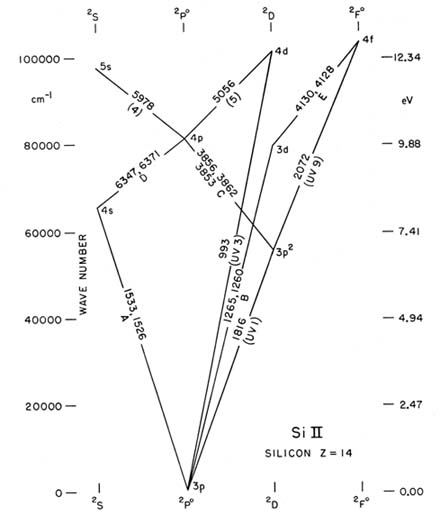
\includegraphics[width=\linewidth]{figures/grotrian-si-ii.jpg}
\caption{The Grotrian diagram for \ion{C}{IV}.}
\label{figure-grotrian-c-iv}
\end{figure}

\begin{figure}
\centering
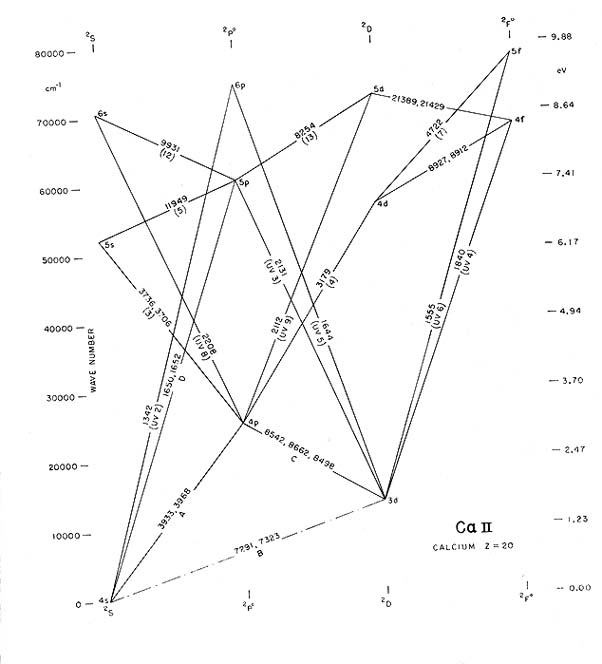
\includegraphics[width=\linewidth]{figures/grotrian-ca-ii.jpg}
\caption{The Grotrian diagram for \ion{Ca}{II}.}
\label{figure-grotrian-ca-ii}
\end{figure}

\begin{table}
\caption{Common Resonance Lines}
\label{table-resonance-lines}
\begin{center}
\begin{tabular}{lll}
\hline
Line& Wavelength& Transition\\
\hline
Ly$\alpha$& \singlet{1216}& $1s$--$2p$\\
\ion{He}{II}& \singlet{304}&\\
\hline
\ion{Li}{I}     &\singlet{6707}         &$2s\:^2\!S$--$2p\:^2\!P^0$\\
\ion{C}{IV}     &\doublet{1548}{1550}   &\\
\ion{N}{V}      &\doublet{1239}{1243}   &\\
\ion{O}{VI}     &\doublet{1032}{1038}   &\\
\hline
\ion{C}{II}     &\doublet{1037}{1036}   &$2p\:^2\!P^0$--$2p^2\:^2\!S$\\
\hline
\ion{C}{II}     &\doublet{1334}{1335}   &$2p\:^2\!P^0$--$2p^2\:^2\!D$\\
\ion{N}{III}    &\doublet{990}{992}     &\\
\hline
\ion{Na}{I} D   &\doublet{5890}{5896}   &$3s\:^2\!S$--$3p\:^3\!P^0$\\
\ion{Mg}{II}    &\doublet{2795}{2802}   &\\
\ion{Al}{III}   &\doublet{1855}{1863}   &\\ 
\ion{Si}{IV}    &\doublet{1394}{1403}   &\\
\hline
\end{tabular}
\end{center}
\end{table}

Why do resonance lines lead to scattering? When a photon is
absorbed in a resonance line, it excites the upper state.
Once in the upper state, there are several posibilities:
radiative decay to the ground state by the permitted
resonance transition, collisional excitation to another
state, a forbidden radiative decay, or a second absorption
leading to a further excitement. Of these possibilities,
radiative decay is dominantly more probable in all cases
except the most extreme densities of particles (in which
collisions can become important) or photons (in which case
further radiative excitements can become important). Thus,
in the conditions encountered in atmospheres, the radiative
excitement of a resonance transition will result in a
subsequent radiative decay of the same resonance transition.
The absorption followed by rapid emission mimics a
scattering process in which photons are conserved. Thus, we
often treat resonance lines within the framework of
scattering, even though at the atomic level we are dealing
with true absorption and true emission.

The scattering coefficient for resonance scattering is
isotropic but, obviously, frequency dependent. We normally
write the scattering coefficient as
\begin{align}
\sigma_\nu(\nu) = \sigma_\mathrm{L}\phi(\nu),
\end{align}
where $\phi$ is normalized such that
\begin{align}
\int_0^\infty\!\!\!d\nu\:\phi(\nu) = 1.
\end{align}
Thus, $\sigma_\mathrm{L}$ determines the strength of the
line and $\phi(\nu)$ determines its shape or
profile.

Resonant line scattering is incoherent and anisotropic.
However, the changes in frequency and direction are
independent. The change in direction is characterized by the
dipole phase function $g$ and the change in frequency is
given characterized by the frequency redistribution function
$p$. We have encountered the phase function previously, but
the frequency redistribution function is new. It is defined
so that $p(\nu',\nu)$ is the probability density that a
scattered photon with frequency $\nu'$ becomes a photon with
frequency $\nu$. It is thus normalized such that
\begin{align}
\int_0^\infty\!\!\!d\nu'\:p(\nu',\nu) =
\int_0^\infty\!\!\!d\nu\:p(\nu',\nu) =
1.
\end{align}
Comparing the definitions and the normalizations, we can
identify
\begin{align}
\Sigma(\nu', \vec n'; \nu, \vec n)
= 
\frac{1}{4\pi}
g(\vec n', \vec n)
p(\nu',\nu),
\end{align}
and so the scattered emissivity is given by
\begin{align}
j_\nu^\mathrm{s}(\nu, \vec n) = 
\frac{1}{4\pi}
\sigma_\mathrm{L}
\int_0^\infty \!\!\! d\nu' 
\int_{4\pi} \!\!\! d\Omega'
\:
\phi(\nu')
p(\nu',\nu)
g(\vec n', \vec n)
I_\nu(\nu', \vec n').
\end{align}

One limiting case is known as complete redistribution in
which there is no correlation between the frequency of the
incoming and scattered photon. We then have $p(\nu',\nu) =
\psi(\nu)$, where $\psi(\nu)$\comment{Have we used $\psi$
and $\phi$?} is the shape of the emission profile and is
 normalized such that
\begin{align}
\int_0^\infty\!\!\!d\nu\:\psi(\nu) = 1.
\end{align}
In general, the absorption and emission profiles of a line
are different, but for complete redistribution we have
$\psi(\nu) = \phi(\nu)$. The scattered emissivity is given
by
\begin{align}
j_\nu^\mathrm{s}(\nu, \vec n) = 
\frac{1}{4\pi}
\sigma_\mathrm{L}
\psi(\nu)
\int_0^\infty \!\!\! d\nu' 
\int_{4\pi} \!\!\! d\Omega'
\:
\phi(\nu')
g(\vec n', \vec n)
I_\nu(\nu', \vec n').
\end{align}
Since $I_\nu$ can be anisotropic and can vary over the line
profile, we cannot in general simplify this integral
further. Complete redistribution is a good approximation in
the line core or when collisions are so frequent that the
energy of the upper state is significantly perturbed before
re-emission of the photon. In general, though, the
frequencies of the incoming and scattered photons are
correlated, and we must use a general redistribution
function $p(\nu',\nu)$.

\section{Dust Scattering}

Dust grains can form in the atmospheres of cool stars. Dust
grains scatter light coherently. The phase function of a
single grain depends on its size, shape, and composition,
and one must average over the distributions of all of these.
The Henyey-Greenstein phase function, although it has no
theoretical basis, is often used to approximate the phase
function for dust scattering. It is given by
\begin{align}
g(\mu_\mathrm{s}) = 
\frac{(1 - \bar\mu_\mathrm{s}^2)}{(1 + \bar\mu_\mathrm{s}^2 - 2
\bar\mu_\mathrm{s}\mu_\mathrm{s})^{3/2}},
\end{align}
The parameter $\bar\mu_\mathrm{s}$ is the mean value of the
scattering angle $\mu_\mathrm{s}$.

\comment{Discussion of $\sigma$. Figure of $g$. $\bar\mu_\mathrm{s}$ is sometimes
called $g$.}

\section{The Isotropic Scattering Approximation}

We have seen that the physically important scattering
mechanisms are anisotropic, and that these lead to an
anisotropic emission coefficientes when the intensity is
anisotropic, as it is in stellar atmospheres. Taking
coherent anisotropic scattering as an example, the emission
coefficient is given by
\begin{align}
j_\nu^\mathrm{s} &= 
\frac{\sigma_\nu(\nu)}{4\pi} 
\int_{4\pi} \!\!\! d\Omega
\:
g(\mu_\mathrm{s}) I_\nu
\end{align}
We can separate the isotropic and anisotropic parts of
$I_\nu$ and $g$ by rewriting them as $J_\nu[1 + (I_\nu-J_\nu)/J_\nu]$
and $1 + (g - 1)$. We then obtain,
\begin{align}
j_\nu^\mathrm{s} =  
\sigma_\nu J_\nu
\left[
1
+ 
\frac{1}{4\pi J_\nu}
\int_{4\pi} \!\!\! d\Omega
\:
(g(\mu_\mathrm{s}) - 1) (I_\nu - J_\nu)\right].
\end{align}
We can see that this is just the scattered emissivity for an
isotropic scatterer, $\sigma_\nu J_\nu$, multiplied by a
normalized correction factor. Furthermore, it allows us see
that we can approximate anisotropic scattering by isotropic
scattering when either the intensity field is not too
anisotropic, that is, when $I_\nu \approx J_\nu$ , or the
scattering is not too isotropic, that is, when $g
\approx 1$. In
effect, near isotropy in the radiation field can compensate
for anisotropy in the scattering and vice versa. Assuming
isotropic scattering significantly simplifies the
calculation of the scattered emissivity, as we can eliminate
integrals over $g$, and also simplifies the radiation
transfer problem, as the scattered emissivity becomes
isotropic and we can ignore its angular dependence.

This approximation will be good deep in the atmosphere,
where the radiation field will become isotropic. At low
optical depths, it is not obviously correct, as the
radiation field becomes significantly anisotropic. However,
the approximation is often used regardless, simply because
an anisotropic emissivity is such a complication. In all
that follows, we will assume that we can replace anisotropic
scattering by isotropic scattering.

Furthermore, Problem~\ref{problem-dipole-scattering}
demonstrates that when the anisotropy in $I_\nu$ is linear
in $\mu$, anisotropic dipole scattering (e.g., electron
scattering, Rayleigh scattering, and resonance line
scattering) results in a isotropic scattering emission
coefficient. This means that where the diffusion
approximation is valid and the specific intensity is linear
in $\mu$, electron scattering and dipole scattering in
general can be exactly treated as isotropic scattering.
Furthermore, in the atmosphere, where the specific intensity
will not in general be linear in $\mu$, any anisotropy in
the scattering emission coefficient arises from second- and
higher-order anisotropies in the specific intensity, and
this gives additional hope that the isotropic scattering
approximation might be good.
\comment{Actually, it's isotropic for all odd-ordered
anisotropies.}

\section{Pure Coherent Scattering Atmosphere}

The simplest atmosphere that involves scattering is one in
which we have only coherent isotropic scattering and no
absorption or emission and in which radiative equilibrium
holds. The only sources of emissivity and extinction are
scattering, so we have $j_\nu = \sigma_\nu J_\nu$ and
$\chi_\nu = \sigma_\nu$. The source function is thus,
\begin{align}
S_\nu \equiv \frac{j_\nu}{\chi_\nu} =
\frac{\sigma_\nu J_\nu}{\sigma_\nu} = J_\nu.
\end{align}
We have seen something very similar in the development of
the grey atmosphere, in which we have $S = J$. Thus, the
pure coherent scattering atmosphere behaves at each
frequency like an integrated grey atmosphere. In particular,
the mean instensity as a function of optical depth is given
by
\begin{align}
J_\nu(\tau_\nu) = 3H_\nu(\tau_\nu + q(\tau_\nu))
\end{align}
and the limb darkening is given by
\begin{align}
\frac{I_\nu(0,\mu)}{I_\nu(0,1)}
=
\frac{H(\mu)}{H(1)}.
\end{align}
These are identical to the results for the grey atmosphere,
except that all quantities explictly depend on $\nu$.

What about the flux? Since scattering is coherent, photons
never change frequency. This implies that $F_\nu$ is
constant with depth, and is determined by the incident flux
on the lower boundary of the atmosphere.

\section{Combined Scattering and Absorption}

We'll now consider the qualitative behaviour of an
atmosphere that combines scattering and absorption. 

Each time a photon is emitted or scattered, it travels on
average one mean free path before being absorbed or
scattered. If we have isotropic scattering, then the photon
will perform a random walk, and if it travels a total of N
free paths, it will have a RMS displacement of $N^{1/2}$
mean free paths from its starting point.

Each time a photon interacts with matter, it is either
absorbed with a probability $\epsilon$ or scattered with a
probability $1-\epsilon$. (The quantity $1-\epsilon$ is
known as the single-scattering albedo.) Thus, the mean
number of mean free paths that the photon travels before it
is absorbed is $1/\epsilon$.

Combining these results, we see that a photon is reabsorbed
on average $1/\sqrt\epsilon$ mean free paths from its point
of emission. In optical depth terms, this corresponds to a
change in optical depth of $\Lambda = 1/\sqrt\epsilon$.
(This $\Lambda$ is not to be confused with the $\Lambda$
operator.) The quantity $\Lambda$ is known as the
thermalization length, diffusion length, or effective mean
path.

If we consider the case of $\epsilon = 1$, in which there is
no scattering, photons are reabsorbed only one mean free
path from their point of emission. This means that the
effects of gradients in the radiation field, caused perhaps
by temperature gradients, are seen only about one optical
depth away, and the radiation transfer problem is relatively
local.

On the other hand, if scattering is important and $\epsilon
\ll 1$, photons will be absorbed on average many mean free
paths from their point of emission. Changes in the radiation
field can be seen many optical depths away. This means, for
example, that the influence of the upper limit of the
atmosphere can be seen many optical depths into the
atmosphere and that parts of the atmosphere that are many
optical depths apart are now coupled. The radiation transfer
problem is now distinctly non-local and becomes distinctly
more difficult. This partly explains why the addition of
strong scattering, most often in the form of resonance
lines, creates such problems.

The name ``thermalization length'' stems, I believe, from
being the length over which a photon travels before it is
absorbed and re-enters the thermal pool of energy. It is
closely connected with the depth at which the source
function approaches $B_\nu$. We will encounter it again when
we study NLTE line formation.

